\documentclass[11pt]{article}
\usepackage[margin=1in]{geometry}
\usepackage{amsmath,amssymb}
\usepackage{newtxtext,newtxmath}
\usepackage{booktabs}
\usepackage{makecell}
\usepackage{siunitx}
\usepackage{graphicx}
\usepackage{caption}
\usepackage[dvipsnames]{xcolor}
\usepackage{microtype}
\usepackage{enumitem}
\captionsetup{font=small,labelfont=bf}
\usepackage[colorlinks=true,allcolors=RoyalBlue]{hyperref}

\newcommand{\Dhat}{\widehat{D}}
\newcommand{\pd}[2]{\partial #1/\partial #2}
\newcommand{\uu}{\times10^{-7}\,\mathrm{s}^{-1}}

\title{\bfseries How array geometry shapes the orientation sensitivity of
glider-derived vertical velocity}
\author{Technical note --- TPOSE24 wave-glider OSSE}
\date{\today}

\begin{document}
\maketitle

\begin{abstract}
\noindent
A small array of wave gliders estimates horizontal divergence---and, through continuity,
vertical velocity $w$---by fitting a plane to the velocities it samples and reading off the
slopes. Because the ocean features drifting through the array arrive at arbitrary
orientations, we ask a design question: \emph{does the estimate depend on how the flow
happens to be oriented relative to the array, and if so, which array shapes are least
sensitive?} We work up from specific cases to the general one. Single-scale test flows turn
out to fool exactly one array shape each and leave every other shape exactly invariant; a
broadband, ocean-like flow fools every shape a little, in a ranking that at first looks
erratic---a pentagon beating a hexagon, a triangle tying it. Averaged over where the array
sits in the flow, however, the ranking becomes strictly monotone in the number of gliders.
All of it follows from one idea: $n$ gliders equally spaced around a ring sample the flow at
$n$ azimuthal points, and like any equally spaced sampling they cannot resolve structure that
repeats a multiple of $n$ times around the ring. The number of gliders therefore sets which
azimuthal scales alias, exactly as a sampling rate sets a Nyquist frequency. Together with
noise, robustness, and footprint considerations, this favors the regular hexagon for a
six-glider array.
\end{abstract}

\section{The estimate and the question}
\label{sec:setup}

Let the gliders sit at horizontal offsets $(x,y)$ (east, north) from the array center, all at
radius $r$ from it, so the array diameter is $d=2r$. The array samples the horizontal velocity
$(U,V)$ and estimates the horizontal divergence
\begin{equation}
  D=\pd{U}{x}+\pd{V}{y},
  \qquad
  w(-H)=-\int_{-H}^{0} D\,\mathrm dz ,
  \label{eq:div}
\end{equation}
the vertical velocity following by integrating continuity down to depth $H$. With only a
handful of point samples, the array fits a plane to each velocity component,
\begin{equation}
  U\approx a_0+a_1x+a_2y,\qquad V\approx b_0+b_1x+b_2y,
  \label{eq:planefit}
\end{equation}
and reads the divergence off the fitted slopes, $\Dhat=a_1+b_2$. A plane has a single,
constant slope, so $\Dhat$ is the array's best single-number estimate of the divergence
averaged over its footprint. Because both the estimate and the average are linear in the
velocity, time-averaging passes straight through them and we may reason about one snapshot at
a time.

The ocean structures that drift through the array---eddies, fronts, wave packets---arrive at
every orientation. So we rotate the flow rigidly by an angle $\theta$ relative to the fixed
array and ask how $\Dhat$ responds. An array whose estimate is independent of $\theta$ is one
whose skill does not depend on the (unknowable) orientation of the passing feature. Throughout
we compare the five regular arrays of Fig.~\ref{fig:polygons}, all at the same radius
$r=\SI{0.75}{\degree}$, so that differences come from the \emph{arrangement} of the gliders
rather than from the size of the array.

\begin{figure}[t]
\centering
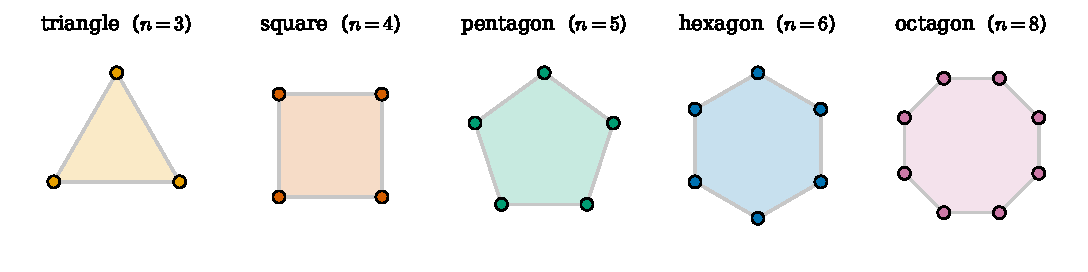
\includegraphics[width=\linewidth]{fig1_polygons.pdf}
\caption{The five regular arrays compared throughout, drawn at a common radius $r$. Only the
number of gliders $n$ and their angular arrangement differ.}
\label{fig:polygons}
\end{figure}

\section{One flow, two arrays}
\label{sec:example}

Start with a single concrete case (Fig.~\ref{fig:example}): a sum of two tilted waves with
structure comparable in scale to the array, sampled by the two candidate OSSE footprints---the
four-corner square and the regular hexagon. The flow (panel a) has a curved divergence field
across the footprint, with a positive core and negative flanks (panel b), so no plane can
reproduce it exactly.

Rotating that flow past the arrays (panel c) shows the effect this note is about. The estimate
is not a fixed number: it depends on the orientation at which the feature arrives. The square's
error swings by $6.4\uu$ peak to peak and cycles \emph{four} times per revolution, with a
smaller ripple at eight cycles superposed; the hexagon swings by only $1.6\uu$---four times
less---and cycles \emph{six} times. Both numbers, four and six, will turn out to be exactly the
glider counts, but let us treat them as measurements for now.

\paragraph{Two things to keep separate.} Both curves in Fig.~\ref{fig:example}(c) are offset
\emph{above} zero (means $+0.9$ and $+0.5\uu$). That offset is the same at every
orientation: it is the error a flat plane makes against a curved field, a scale-matching
problem set by array size (\S\ref{sec:other}), and it has nothing to do with orientation. The
\emph{swing} about that offset is the orientation sensitivity. From here on we measure the
swing as the peak-to-peak range of $\Dhat(\theta)$ about its own rotational mean, which
isolates the orientation dependence and requires no choice of reference truth; it is also
directly comparable between shapes whose footprints enclose different areas. Panel (c) is the
one place we grade against the truth (each array's own footprint average), because there the
offset itself is worth seeing.

\begin{figure}[t]
\centering
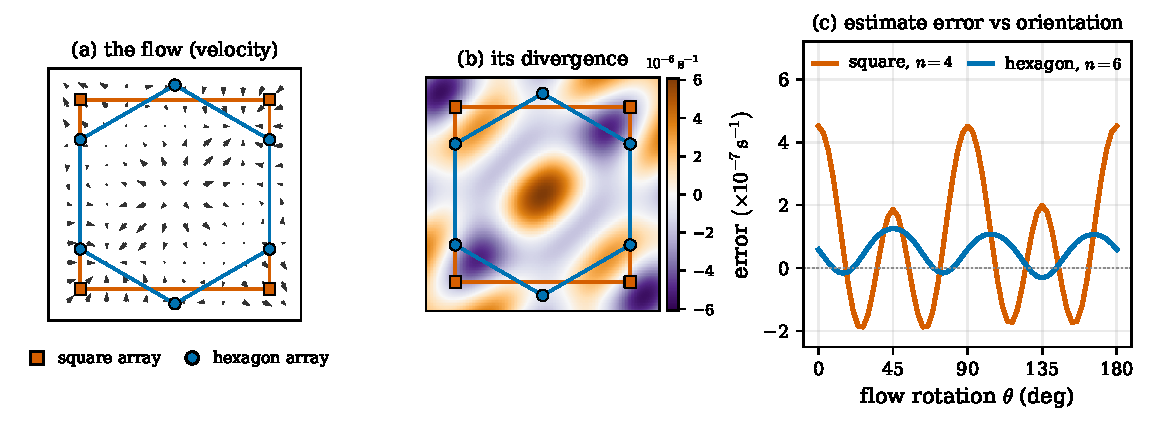
\includegraphics[width=\linewidth]{fig2_example.pdf}
\caption{A worked example. \emph{(a)} A two-scale wave flow, with the four-corner square array
(\SI{1.5}{\degree} box) and the regular hexagon drawn on top. \emph{(b)} Its true divergence,
which is curved across both footprints. \emph{(c)} Error of each array's plane-fit
divergence---estimate minus the true average over that array's own footprint---as the flow is
rotated through \SI{180}{\degree}. The square cycles four times and swings four times further
than the hexagon, which cycles six times. The common offset above zero is the
orientation-independent bias of a plane fit to a curved field.}
\label{fig:example}
\end{figure}

\section{Single-scale flows: each fools exactly one shape}
\label{sec:single}

Next take flows simple enough to isolate one behavior at a time (Table~\ref{tab:cases}) and run
all five arrays through a full rotation (Fig.~\ref{fig:curves}). The results are unusually
clean.

\begin{itemize}[nosep,leftmargin=1.4em]
\item A flow with a \textbf{uniform gradient} is reproduced perfectly by every array at every
orientation. A plane fit is exact for a field that really is a plane, so the first thing it can
get wrong is \emph{curvature}.
\item The \textbf{curvature} flow moves the \emph{triangle} and nothing else. The triangle's
estimate cycles three times per revolution; the square, pentagon, hexagon and octagon are flat
to machine precision---exactly invariant.
\item The two \textbf{cubic} flows move the \emph{square} and nothing else, cycling four times
per revolution (period \SI{90}{\degree}), in opposite phase to each other. The triangle,
pentagon, hexagon and octagon are again exactly invariant.
\end{itemize}

The headline is counter-intuitive: the square---the roundest-looking four-point array---is the
\emph{only} regular polygon that fails the cubic flows, and it fails them precisely because its
four-fold symmetry matches something four-fold in the flow. Symmetry that matches the flow is a
liability, not an asset. Note also the pattern in Table~\ref{tab:cases}: whether the velocity
reverses sign across the array center decides whether the flow has an even or an odd number of
lobes, and that in turn decides which shape it catches. We come back to this in
\S\ref{sec:mechanism}; it is the single most consequential fact in the note.

\begin{table}[b]
\centering
\small
\setlength{\tabcolsep}{6pt}
\renewcommand{\arraystretch}{1.35}
\begin{tabular}{@{}llccl@{}}
\toprule
Test flow (case) & $U$ \;($V$: swap $x\!\leftrightarrow\! y$) &
\makecell{reverses across\\the center?} & \makecell{error cycles per\\flow revolution} &
\makecell{shape it fools} \\
\midrule
uniform gradient (linear) & $U=S\,x$ & yes & --- & none --- plane fit is exact \\
curvature (even)          & $U=C\,x^{2}$ & \textbf{no} & $3$ & \textbf{triangle} \\
cubic (odd)               & $U=C\,x^{3}$ & yes & $4$ & \textbf{square} \\
cubic + cross-term (mixed)& $U=C\,(x y^{2}+\tfrac12 x^{3})$ & yes & $4$ & \textbf{square} \\
single wave (fine)        & $U=C\sin(Kx+By)$ & yes & $2,4,6,\dots$ & every shape (a little) \\
two waves (combo)         & sum of two such waves & yes & $2,4,6,\dots$ & every shape \\
\bottomrule
\end{tabular}
\caption{The synthetic test flows, and what is \emph{observed} when each is rotated past the
five arrays. ``Error cycles per flow revolution'' is read directly off Fig.~\ref{fig:curves}.
Nothing here is theory yet: the last two columns are measurements.}
\label{tab:cases}
\end{table}

\begin{figure}[t]
\centering
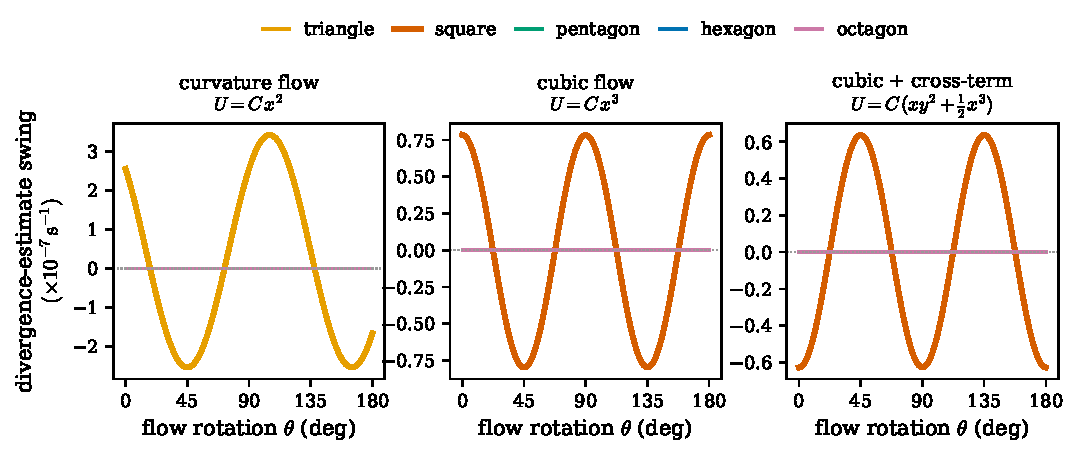
\includegraphics[width=\linewidth]{fig3_rotation_curves.pdf}
\caption{Divergence-estimate swing versus the flow-rotation angle $\theta$ for the three
polynomial flows, all five arrays overlaid. The triangle alone oscillates for the
\emph{curvature} flow; the square alone oscillates for the \emph{cubic} and
\emph{cubic\,+\,cross-term} flows, in opposite phase; every other array is flat---exactly
invariant, to machine precision. Bold curves mark the shape that is fooled in each panel.}
\label{fig:curves}
\end{figure}

\section{Broadband flow at one placement}
\label{sec:broadband}

Real ocean flow is not single-scale. Returning to the two-scale wave field of
\S\ref{sec:example}---still with the array centered exactly as in Fig.~\ref{fig:example}---no
array is exactly invariant any more, and the ranking (blue bars in
Fig.~\ref{fig:features}a) looks erratic:
\begin{center}
\small
\begin{tabular}{@{}lccccc@{}}
\toprule
 & triangle & square & pentagon & hexagon & octagon \\
swing ($\uu$) & $3.66$ & $9.81$ & $0.15$ & $3.66$ & $3.02$ \\
\bottomrule
\end{tabular}
\end{center}
The square is by far the worst. The pentagon is essentially silent. The triangle---three
gliders---ties the six-glider hexagon \emph{exactly}, to five decimal places. This is not what
one expects from ``more gliders is better,'' and it is worth being suspicious of: the ranking is
not monotone in $n$, and one of these numbers is about to turn out to be an accident.

\paragraph{Adding a centered feature.} Real flow also contains features the array straddles
whose velocity does not reverse across the center---a jet core, an eddy center. Adding one to
the wave field, scaled to the same RMS speed (red bars, Fig.~\ref{fig:features}a), raises the
triangle's swing from $3.66$ to $12.3\uu$ and leaves the square, pentagon, hexagon and octagon
\emph{numerically unchanged}. Which shape responds is a property of the geometry; how large the
response is depends on how energetic the feature happens to be, and
Fig.~\ref{fig:features}(b) sweeps that: four flat lines and one rising one, with the triangle
overtaking the square only past about $0.75$ of the wave field's RMS speed. So the honest claim
is not ``the triangle is the worst shape''---in this flow the square is worse until the feature
is strong---but that the triangle is the only array a centered feature can touch at all.

\begin{figure}[t]
\centering
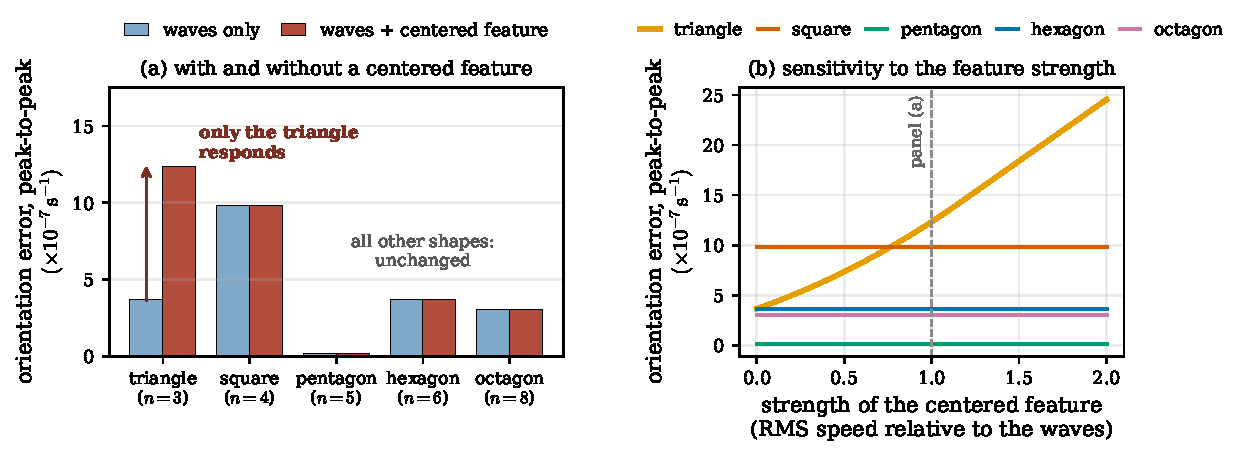
\includegraphics[width=\linewidth]{fig4_features.pdf}
\caption{Orientation error (peak-to-peak swing over a full flow rotation) for the broadband,
two-scale wave field at the centered placement, with and without a centered feature (a jet/eddy
core, whose velocity does not reverse across the array). \emph{(a)} Adding the feature raises
the error of \emph{only} the triangle; the other four are unchanged to machine precision. Note
that the square is nonetheless the loudest shape on the waves alone, and that the ranking is not
monotone in $n$. \emph{(b)} The same error as the feature's strength is swept: four shapes are
flat---geometrically insensitive to it---while the triangle rises and overtakes the square at
about $0.75$. Which shape responds is set by geometry; which is worst overall is set by the
flow.}
\label{fig:features}
\end{figure}

\section{The general case: many placements}
\label{sec:general}

The suspicious numbers in \S\ref{sec:broadband} come from one particular placement: the array
sitting exactly on the center of the wave field, straddling a zero crossing, so that the
velocity it sees reverses across the array. That is a symmetric special case, and the ocean has
no reason to oblige.

Before averaging anything, take one specific alternative. Displace the array by
$(0.37\si{\degree},0.21\si{\degree})$---about a third of the dominant wavelength, so that it no
longer straddles the zero crossing---and run the identical rotation experiment in the identical
flow:
\begin{center}
\small
\begin{tabular}{@{}lccccc@{}}
\toprule
 & triangle & square & pentagon & hexagon & octagon \\
\midrule
centered, from \S\ref{sec:broadband} & $3.66$ & $9.81$ & $0.15$ & $3.66$ & $3.02$ \\
displaced ($\uu$)                    & $4.16$ & $7.84$ & $6.14$ & $2.10$ & $1.36$ \\
\bottomrule
\end{tabular}
\end{center}
The pentagon goes from the quietest shape to the second loudest---$0.15$ to $6.14$, a factor of
forty---and now loses to the hexagon three times over. The triangle's exact tie with the hexagon
is gone as well ($4.16$ against $2.10$). Nothing about the arrays changed between these two rows:
same shapes, same radius, same flow, same rotation. Only where the array sits in the field
changed. Whatever produced the striking ranking of \S\ref{sec:broadband}, it was not a property
of the shapes.

Figure~\ref{fig:ensemble} does this systematically, for 400 random placements of each array in
the same wave field. Averaged over placement, the ranking is strictly monotone in the number of
gliders:
\begin{center}
\small
\begin{tabular}{@{}lccccc@{}}
\toprule
 & triangle ($n=3$) & square ($4$) & pentagon ($5$) & hexagon ($6$) & octagon ($8$) \\
mean swing ($\uu$) & $8.64$ & $6.12$ & $4.04$ & $3.09$ & $1.60$ \\
\bottomrule
\end{tabular}
\end{center}
Two of the puzzles from \S\ref{sec:broadband} dissolve. The pentagon's near-silence
($0.15$) was a property of that one placement, not of the shape: over the ensemble it averages
$4.04$ and loses to the hexagon, as the glider count says it should. And the triangle's tie with
the hexagon was likewise placement-specific---in general the triangle is the \emph{worst} of the
five, at more than twice the hexagon's error. The stars in Fig.~\ref{fig:ensemble} mark the
special placement: lucky for the triangle and pentagon, unlucky for the square and octagon, and
representative for none of them.

This is the practically important statement. If an array could be guaranteed to sit centered on
the features it measures, shape would matter in the intricate way \S\ref{sec:broadband}
suggests. It cannot, so what matters is the ensemble: \emph{more gliders, monotonically better},
with the triangle worst.

\begin{figure}[t]
\centering
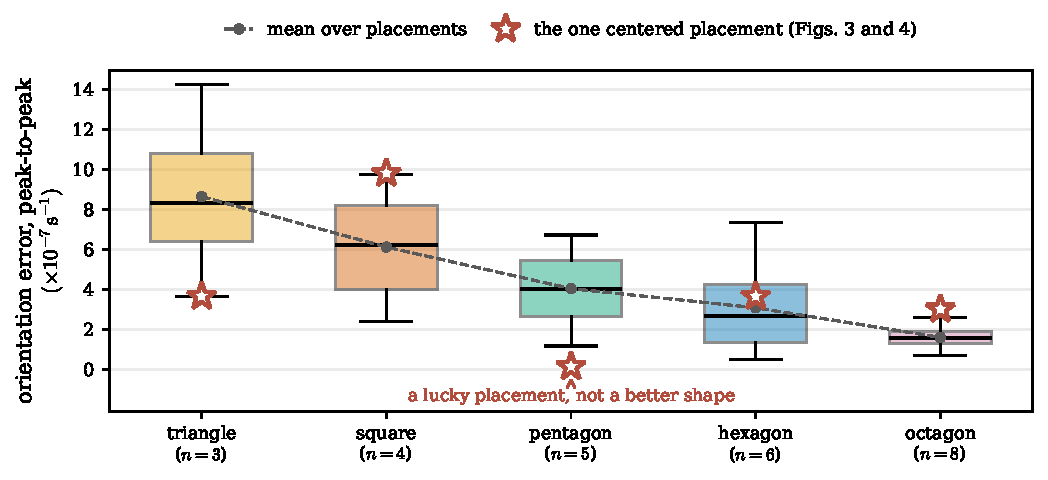
\includegraphics[width=\linewidth]{fig5_ensemble.pdf}
\caption{Orientation error over 400 random placements of each array within the same two-scale
wave field (boxes: median and interquartile range; whiskers: 5th--95th percentiles). Averaged
over placement the ranking is monotone in the number of gliders, and the pentagon's apparent
advantage in Fig.~\ref{fig:features} disappears. Stars mark the single centered placement used
in Figs.~\ref{fig:curves} and~\ref{fig:features}, which is an outlier for four of the five
shapes.}
\label{fig:ensemble}
\end{figure}

\section{Why: the array as an azimuthal sampler}
\label{sec:mechanism}

One idea accounts for every result above. Picture the flow's structure as seen going once around
the ring of gliders. It has some azimuthal pattern, which we decompose into modes that repeat
$m$ times per lap---$m$ is the azimuthal wavenumber, familiar from wavenumber-1 and
wavenumber-2 asymmetries in a vortex; $m=0$ is uniform.

\begin{figure}[t]
\centering
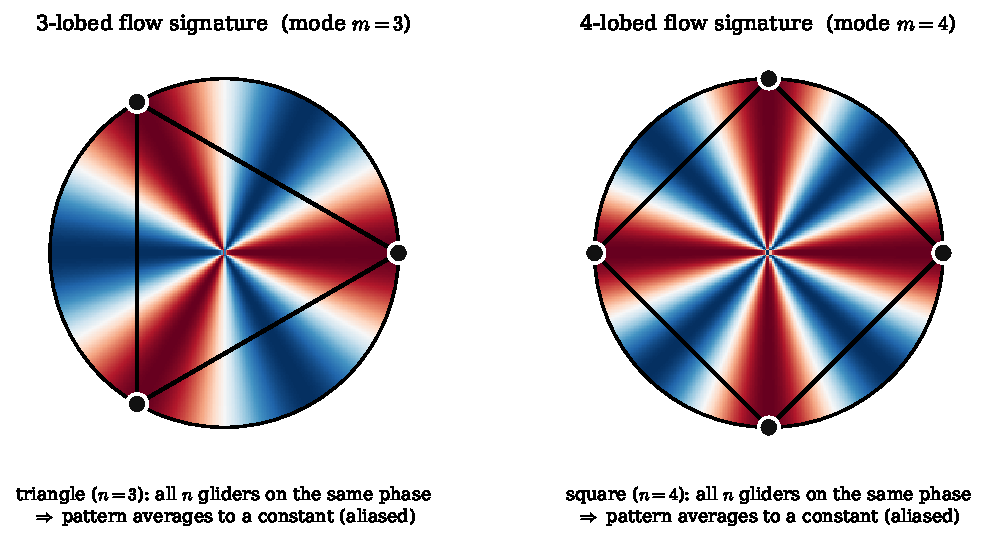
\includegraphics[width=0.82\linewidth]{fig6_aliasing.pdf}
\caption{Why a matched flow aliases. \emph{Left:} a three-lobed flow signature ($m=3$) sampled
by a triangle---all three gliders sit at the same phase (here, all on a red lobe), so the
three-lobed pattern is indistinguishable from a uniform one and contaminates the divergence
estimate. \emph{Right:} the same for a four-lobed signature ($m=4$) sampled by a square. Each
regular array is blind precisely to the wavenumber that matches its glider count.}
\label{fig:aliasing}
\end{figure}

\paragraph{Equally spaced samples alias.} Because $n$ gliders sit at equal angular spacing,
summing any azimuthal mode around the ring cancels it \emph{unless} the mode repeats a whole
number of times between neighboring gliders---that is, unless $m$ is a multiple of $n$. This is
the rotational form of the Nyquist statement: equally spaced samples cannot distinguish
structure at multiples of the sampling rate from a constant, and alias it. A regular $n$-glider
array therefore \emph{reproduces the true divergence for any flow with no structure at
$m=n,2n,3n,\dots$}, and is fooled only at those \emph{blind modes}. Figure~\ref{fig:aliasing}
shows the mechanism directly: when the flow's lobes line up with the gliders, every glider reads
the same phase, the pattern is indistinguishable from a uniform one, and it leaks into the
divergence estimate.

As the flow rotates, the aliased modes sweep past the gliders and the estimate oscillates:
\begin{equation}
  \Dhat(\theta)=D_{\text{true}}+\sum_{j\ge1} a_{jn}\,\cos\!\big(jn\,\theta-\varphi_{jn}\big)
  \;\approx\; D_{\text{true}}+a_{n}\cos\!\big(n\theta-\varphi_n\big),
  \label{eq:alias}
\end{equation}
where $a_m$ is the strength of the flow's structure at wavenumber $m$. The sum runs only over
multiples of $n$, and because a smooth flow's $a_m$ fall off with $m$, the lowest surviving term
dominates. This is why the square's error in Fig.~\ref{fig:example} cycles four times per
revolution and the hexagon's six: the cycle count \emph{is} the glider count.

\medskip
\noindent\fbox{\parbox{0.965\linewidth}{A regular $n$-glider array's orientation error is set by
how much of the flow's structure repeats exactly $n$ times around the ring. More gliders push
that blind mode to higher $m$, where a smooth flow carries less energy---the rotational form of
anti-aliasing.}}

\paragraph{Wavenumber and physical scale.} Azimuthal wavenumber ties to physical scale through
the array size: a feature of horizontal wavelength $\lambda$ wrapped around a ring of diameter
$d$ registers at
\begin{equation}
  m\approx \frac{2\pi r}{\lambda}=\frac{\pi d}{\lambda}.
  \label{eq:scale}
\end{equation}
Features much larger than the array ($\lambda\gg d$) sit at low wavenumber and are handled
cleanly; features comparable to or smaller than the array reach $m\gtrsim3$ and begin to alias
on the smallest arrays. Two design levers follow: adding gliders raises the blind mode
(Eq.~\ref{eq:alias}), and shrinking the array raises the wavelength at which a given feature
aliases (Eq.~\ref{eq:scale}), at the cost of a shorter baseline and noisier slopes
(\S\ref{sec:other}).

\paragraph{Parity, and why the pentagon looked good.} Here is the fact flagged in
\S\ref{sec:single}. If the velocity \emph{reverses} across the array center, the flow's
signature contains only even wavenumbers, $m=2,4,6,\dots$; if it does \emph{not} reverse---a
centered jet or eddy core---it contributes odd ones, $m=1,3,5,\dots$. Now combine that with the
blind-mode rule. For a flow that reverses, an array with an \emph{odd} number of gliders is
blind at $m=n$ but the flow has nothing there, so its lowest \emph{active} blind mode is $2n$;
an array with an \emph{even} number is exposed at $n$ itself. Table~\ref{tab:modes} works this
out, and it explains \S\ref{sec:broadband} exactly: at the centered placement the error is
ordered by lowest active mode, not by $n$. The pentagon is quietest because it is not exposed
until $m=10$; the triangle ties the hexagon because both are first exposed at $m=6$; the square
is worst because it is exposed at $m=4$.

Figure~\ref{fig:spectrum} shows this happening, rather than merely asserting it. Panel (a) is the
azimuthal spectrum of what the array actually samples---the scalar $xU+yV$ around the glider
ring, whose wavenumber-$m$ amplitude is what Eq.~\eqref{eq:alias} turns into an orientation
swing, so the vertical axis is plotted directly in swing units and each array's error can be
read off at $m=n$. Centered on the field (blue), the spectrum is \emph{exactly} zero at every odd
wavenumber: there is nothing at $m=3$ for the triangle to alias and nothing at $m=5$ for the
pentagon, so both are silent at their own blind modes and only respond at $m=6$ and $m=10$
respectively. That is the whole explanation of \S\ref{sec:broadband}, including the exact
triangle--hexagon tie: both are driven by the same $m=6$ amplitude. Displace the array (red) and
the odd wavenumbers fill in---$m=1$ becomes the single largest component---and the pentagon
inherits a substantial $m=5$. Panel (b) confirms that this accounts for the measurements: the
swing predicted from the lowest blind mode carrying any signal (black dashes) reproduces the
measured error shape by shape, at both placements.

So, to answer the question directly: \emph{the pentagon does not beat the hexagon in general.} It
beats it only for flow that is antisymmetric about the array center, a symmetry no real
deployment can count on, and the advantage vanishes as soon as the array is displaced by a
fraction of a wavelength. The same caveat cuts the other way for the triangle: its tie with the
hexagon is the same accident, and a centered feature---the very thing that breaks the
symmetry---exposes it at $m=3$, the lowest blind mode of any shape considered here.

\begin{figure}[t]
\centering
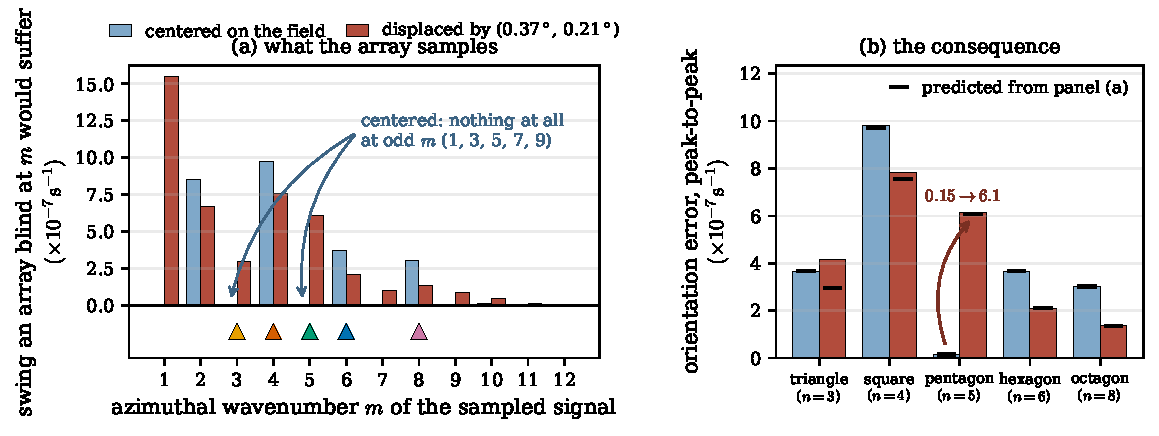
\includegraphics[width=\linewidth]{fig7_spectrum.pdf}
\caption{Why parity decides the ranking, and what changes when the array moves. \emph{(a)}
Azimuthal spectrum of the signal the array samples ($xU+yV$ around the ring), plotted in swing
units so that an array whose lowest active blind mode is $m$ suffers the plotted error;
triangles below the axis mark each array's first blind mode $m=n$, colored as in
Fig.~\ref{fig:polygons}. Centered on the wave field
(blue) there is \emph{no} odd-$m$ content at all, so the triangle ($m=3$) and pentagon ($m=5$)
are blind at wavenumbers the flow does not carry; displaced by
$(0.37\si{\degree},0.21\si{\degree})$ (red), odd wavenumbers appear. \emph{(b)} The consequence
shape by shape, with the swing predicted from panel (a) marked in black. The pentagon's error
rises by a factor of forty. The one visible gap---the displaced triangle---is where two blind
modes ($m=3$ and $m=6$) contribute comparably and the leading term alone undershoots.}
\label{fig:spectrum}
\end{figure}

\begin{table}[t]
\centering
\small
\setlength{\tabcolsep}{7pt}
\renewcommand{\arraystretch}{1.3}
\begin{tabular}{@{}lccccccc@{}}
\toprule
& & & \multicolumn{2}{c}{centered placement (\S\ref{sec:broadband})}
& & \multicolumn{2}{c}{general placement (\S\ref{sec:general})} \\
\cmidrule(lr){4-5}\cmidrule(lr){7-8}
array & $n$ & blind modes & \makecell{lowest\\active $m$} & \makecell{swing\\($\uu$)}
& & \makecell{lowest\\active $m$} & \makecell{mean swing\\($\uu$)} \\
\midrule
triangle & 3 & $3,6,9,\dots$  & $6$  & $3.66$ & & $3$ & $8.64$ \\
square   & 4 & $4,8,12,\dots$ & $4$  & $9.81$ & & $4$ & $6.12$ \\
pentagon & 5 & $5,10,15,\dots$& $10$ & $0.15$ & & $5$ & $4.04$ \\
hexagon  & 6 & $6,12,18,\dots$& $6$  & $3.66$ & & $6$ & $3.09$ \\
octagon  & 8 & $8,16,24,\dots$& $8$  & $3.02$ & & $8$ & $1.60$ \\
\bottomrule
\end{tabular}
\caption{Why the ranking changes between \S\ref{sec:broadband} and \S\ref{sec:general}. At the
centered placement the flow reverses across the array, so only even wavenumbers are present and
an odd-$n$ array is not exposed until $m=2n$; the measured swing then orders by lowest active
mode ($m=4$ loudest, $m=10$ quietest), not by $n$. At a general placement odd wavenumbers are
present too, every array is exposed at $m=n$, and the swing orders by glider count.}
\label{tab:modes}
\end{table}


\section{What else sets the error, and robustness to array shape}
\label{sec:other}

The aliasing picture governs the \emph{orientation} sensitivity. Two other contributions do not
depend on orientation and should not be conflated with it:
\begin{itemize}[nosep,leftmargin=1.4em]
\item \textbf{The uniform ($m=0$) bias.} A flat plane cannot equal the footprint average of a
\emph{curved} divergence field, independent of orientation or glider count---the offset seen in
Fig.~\ref{fig:example}(c). This is a scale-matching error (array size versus feature size),
reduced by shrinking the footprint (Eq.~\ref{eq:scale}) or by fitting curvature rather than a
plane, which requires more than three gliders.
\item \textbf{Noise.} Random per-glider velocity error of variance $\sigma^2$ propagates to
$\mathrm{Var}(\Dhat)\approx 4\sigma^2/(n\,r^2)$: doubling from three gliders to six halves the
variance. A triangle is exactly determined (three points fix a plane, no redundancy); a hexagon
is over-determined and averages the noise down.
\end{itemize}
Finally, the invariance results are robust to array \emph{shape}, not just to regular polygons.
An axis-aligned stretch of a hexagon---the same six-glider pattern squeezed in latitude---remains
exactly invariant to the cubic flow at \emph{any} elongation; the mechanism-test footprint, which
uses a square bounding box (and so is a stretched, non-regular hexagon), inherits the invariance.
Regularity is convenient but not required; what matters is the angular arrangement of the
gliders.

\section{Design guidance for a six-glider array}
\label{sec:design}

With six gliders one could deploy a single regular hexagon or, say, two triangles. Section
\ref{sec:broadband} appears to tie a single triangle with the hexagon, but \S\ref{sec:general}
shows that tie to be an artifact of a symmetric placement; averaged over placement the triangle
is the worst shape tested. Four arguments point the same way:
\begin{enumerate}[leftmargin=1.5em,nosep]
\item \textbf{Exposure at the lowest wavenumber.} In general flow the triangle is exposed at
$m=3$, lower than any other shape here, and a centered feature---a jet or eddy core the array
straddles---drives exactly that mode (Fig.~\ref{fig:features}). The hexagon rejects everything
below $m=6$.
\item \textbf{Noise.} The hexagon has half the variance of a triangle's divergence estimate
(\S\ref{sec:other}) and, being over-determined, is not at the mercy of a single bad sample.
\item \textbf{Robustness.} Losing one glider leaves the hexagon with five points (a sound plane
fit); it leaves a triangle with two (no fit at all).
\item \textbf{Footprint and bias.} The hexagon spans about twice the area of an inscribed
triangle and, with six points, can fit curvature to attack the uniform-mode bias that three
points cannot resolve.
\end{enumerate}
Two equilateral triangles at the same radius rotated by \SI{60}{\degree} \emph{are} a regular
hexagon; at different radii they leave a three-lobed blind spot and are strictly worse. The
recommended six-glider footprint is the regular hexagon---the shape already adopted by the OSSE's
symmetric-array family.

\section{Summary}
\label{sec:summary}

A glider array's plane-fit divergence is an azimuthal sampler. Worked from the specific to the
general: a single-scale flow fools exactly one array shape and leaves the rest exactly
invariant; a broadband flow at one symmetric placement produces a ranking that is not monotone
in glider number, with a pentagon beating a hexagon and a triangle tying it; and averaging over
where the array sits in the flow---the case that matters for a real deployment---restores a
strictly monotone ordering, more gliders being better, with the triangle worst. The mechanism
behind all three is that $n$ equally spaced gliders cannot resolve structure repeating a
multiple of $n$ times around the ring, so the array is blind at $m=n,2n,\dots$ and its
orientation error is set by the flow's energy at the lowest of these. Whether the velocity
reverses across the array center decides whether the flow carries even or odd wavenumbers, which
is what makes the symmetric placement special and its ranking misleading. Noise, robustness, and
footprint all favor spreading six gliders into a regular hexagon.

\appendix
\section*{Appendix: the aliasing condition}
\label{sec:appendix}

For completeness: writing the plane-fit divergence as a weighted sum of the sampled velocities
and expanding the flow in azimuthal modes $e^{\mathrm i m\varphi}$, the estimate picks up the
flow's wavenumber-$m$ amplitude weighted by $\sum_k e^{\mathrm i m\psi_k}$, the sum over glider
angles $\psi_k$. For $n$ gliders at equal spacing this sum vanishes unless $m$ is a multiple of
$n$, which is the statement of \S\ref{sec:mechanism} and Eq.~\eqref{eq:alias}. (Equivalently,
the array's orientation error is governed by the vertex sums $\sum_k (x_k+\mathrm i y_k)^m$,
which vanish for a regular $n$-gon unless $n$ divides $m$.)

\end{document}
